\begin{exercise}{8}

  \begin{subexercise}
    \begin{enumerate}
      \item $shorterTeammate(X,Y):-\,\, teamNBA(A), player(X,A), player(Y,A), taller(Y,X). $
      \item $neitherCoachNorPlayer(X,Y):-\,\, teamNBA(Y), \text{NOT } coarch(X,Y),
            \text{NOT } player(X,Y).$ \\
            $coachOrPlayer(X,Y):-\,\, teamNBA(Y), NOT neitherCoachNorPlayer(X,Y). $
      \item $coachTallest(X,Y):-\,\, teamNBA(Y), coach(X,Y), player(A,Y), taller(X,A). $
    \end{enumerate}
  \end{subexercise}
  
  \begin{subexercise}
    \begin{enumerate}
      \item
        The graph below is a possible strati graph of the program, where rules
        that are colser to the top have greater stratifaction numbers than rules
        closer to the bottom. Rules that are from the horizontal perspective on
        the same level have the same stratifaction number. \\
        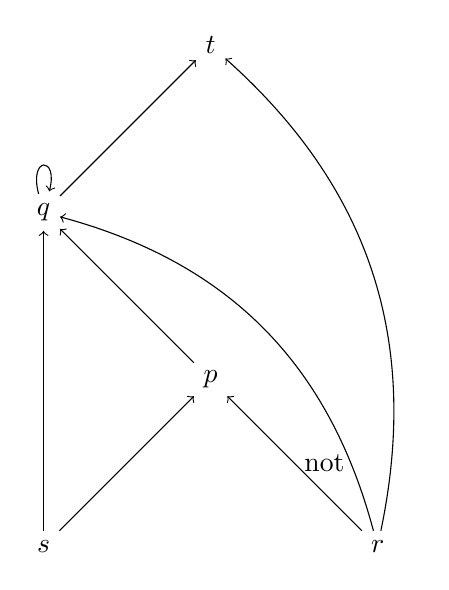
\begin{tikzpicture}[node distance=3cm]
          \node   (t)   {$t$};
          \node   (q) [below left of=t] {$q$};
          \node   (p) [below right of=q]  {$p$};
          \node   (s) [below left of=p] {$s$};
          \node   (r) [below right of=p] {$r$};
%          \node   (v0)  [right of=r]    {$1$};
%          \node   (v1)  [above of=v0]    {$2$};
%          \node   (v2)  [above of=v1]    {$3$};

          \path (q) edge[->,loop above]  node{}  (q)
                    edge[->]  node{} (t);
          \path (p) edge[->]  node{} (q);
          \path (s) edge[->]  node{} (q)
                    edge[->]  node{} (p);
          \path (r) edge[->]  node[above,right]{not} (p)
                    edge[->, bend right]  node{} (q)
                    edge[->, bend right]  node{} (t);
        \end{tikzpicture}
        \\
        Since ther is no rule that uses a rule with a higher stratifaction
        number than its own, the program is stratifiable.

      \item
        \begin{tabular}{l l}
            Herbrand Base & $s(a,b),\,s(b,c),\,s(c,b),\,r(a),\,r(c),\,r(d)$\\
            First application of $T_D$: & $s(a,b)\in F,r(b)\not\in F \rightarrow
                            p(a,b)$ is derivable \\
                                        & $s(b,c)\in F, r(c)\in F \rightarrow
                            p(b,c)$ is not derivable \\
                                        & $s(c,b)\in F, r(b)\not\in F
                            \rightarrow p(c,b)$ is derivable \\
                                        & $p(X,Y) \not \in F$ and $q(X,Y) \not
                                        \in F \rightarrow q(X,Y)$ cannot be
                                        derived \\
                                        & $q(X,Y) \not\in F \rightarrow t(X,Y)$
                                        cannot be derived \\  \\
                              & $F_1 = F \cup \{p(a,b)\} \cup \{p(c,b)\}$ \\ \hline

            Second application of $T_D$:  & $p(a,b)\in F_1, s(b,a)\not\in F_1
                            \rightarrow q(b,a)$ cannot be derived \\
                                          & $p(c,b)\in F_1, s(b,c)\in F_1
                            \rightarrow q(b,c)$ can be derived \\
                                          & $q(X,Y)\not\in F_1 \rightarrow$ no
                                          additional $q(X,Y)$ can be derived \\
                                          & $q(X,Y) \not\in F_1 \rightarrow t(X,Y)$
                                          cannot be derived \\  \\

                              & $F_2 = F \cup \{p(a,b)\} \cup \{p(c,b)\} \cup
                              \{q(b,c)\}$ \\ \hline
            Third application of $T_D$: & $q(b,c)\in F_2, r(a)\in F_2
                          \rightarrow q(b,c)$ can be derived \\
                                        & $q(b,c)\in F_2, r(b)\not\in F_2
                          \rightarrow t(b,c)$ cannot be derived \\ \\

                              & $F_3 = F \cup \{p(a,b)\} \cup \{p(c,b)\} \cup
                              \{q(b,c)\} \cup \{q(c,b)\}$ \\ \hline
            Fourth application of $T_D$: & $q(c,b)\in F_3, r(c)\in F_3
                          \rightarrow t(c,b)$ can be derived \\
                          & all $q(X,Y)$ that could used to dereive a new
                          $t(X,Y)$ were used allready\\
                          &$\rightarrow$ no additional $t(X,Y)$ can be derived\\
                          \\
                          & $F_4 = F \cup \{p(a,b)\} \cup \{p(c,b)\} \cup
                          \{q(b,c)\} \cup \{q(c,b)\} \cup \{t(c,b)\}$ \\ \hline

            Fiveth application of $T_D$ & Since $t(c,b)$ cannot be used to
                        derive anything new\\ & nothing new can be derived \\ \\
                          & $F_5 = F_4 = F \cup \{p(a,b)\} \cup \{p(c,b)\} \cup
                          \{q(b,c)\} \cup \{q(c,b)\} \cup \{t(c,b)\}$ \\ \hline
        \end{tabular}
        \\ \\ Since the only $t-fact$ that can be derived is $t(c,b)$ the only anwser
        is $t(c,b)$.
    \end{enumerate}
  \end{subexercise}

\end{exercise}
